\documentclass[10pt,preprint]{aastex}
\usepackage{amsmath}
\usepackage{breqn}
\usepackage{cite,natbib}
\usepackage{natbib}
\usepackage{epsfig}
\usepackage{cases}
\usepackage[section]{placeins}
\usepackage{graphicx, subfigure}
\usepackage{color}
\usepackage{amsmath}
\usepackage{float}
\floatplacement{figure}{H}
% \usepackage[nomarkers,figuresonly]{endfloat}

\newcommand{\logg}{log \emph{g}~}
\newcommand{\teff}{$T_{eff}~$}
\newcommand{\prot}{$P_{rot}~$}

\newcommand{\ah}{$\hat{A}_n$}
\newcommand{\ph}{$\hat{P}_n$}
\newcommand{\ch}{$\hat{C}_n$}
\newcommand{\gh}{$\hat{G}_n$}
\newcommand{\yh}{$\hat{Y}_n$}
\newcommand{\teffh}{$\hat{T}_n$}

\newcommand{\feh}{[Fe/H]}
\newcommand{\dd}{\ensuremath{\,\mathrm{d}}}

\begin{document}

\section{Rotation Period Measurements}
\label{sec:rotation_period_measurement}

The Kepler light curves of the 505 asteroseismic targets display quasi-periodic variations on timescales corresponding to rotational periods of the stars.
Flux variations are produced by active regions on the stellar surface, rotating in and out of view.
In order to measure periodic signals in the light curves we used the auto-correlation function (ACF) method, developed by \citet{McQuillan2013}.
An autocorrelation function describes the self-similarity of a light curve at a range of lags and the highest peak in the ACF (usually also the first peak) is centered on the dominant periodic signal in the time series.
As an alternative to the standard Fourier decomposition and least-squares fitting of sinusoidal models \citep{Zechmeister}, autocorrelation is better suited to signals that are not sinusoidal or strictly periodic and is more effective at distinguishing a true signal from its harmonics and sub-harmonics.
For a more detailed description of the advantages of the ACF method over sine-fitting periodograms, see \citet{McQuillan}.

Long cadence PDC-MAP data were used throughout this analysis (\citet{Smith_2012}, \citet{Stumpe_2012}).
The PDC-MAP data are the product of an initial systematics removal process applied by the Kepler team, in which large-scale linear trends are removed in order to improve planet transit search and modelling capability.
PDC-MAP data are not, however, optimised to preserve stellar variability: periodic signals longer than around 30 days are reduced in power.
Additionally, light curves still contain large systematic features, such as the exponential decays that appear after telescope shutdowns, which affect period measurement precision.
The Astrophysically Robust Correction (ARC), a detrending method developed by \citet{Roberts2013}, is better at preserving astrophysical signals, however, it has not yet been applied to all Kepler quarters, so we opt to use PDC-MAP.
% {\color{red} So why are we still using it then?! - explain!}
% Note - I HAVE done some injection tests... could talk about these, although it would probably involve quite a lot more work...

In our implementation of the ACF method the first two peaks in the ACF were identified and the central value of the first peak was temporarily accepted as the period (unless the second peak was higher than the first in which case {\it its} central value was taken).

Note that an important advantage of the ACF method over a periodogram approach is in its ability to differentiate between harmonic signals produced by multiple active regions on the stellar surface from the true periodic signal: these scenarios usually produce ACFs in which the second peak is higher than the first.
Subsequent peaks in the ACF lying within 10\% of an integer multiple of the period were identified.
The final, reported period is calculated from the mean separation between peaks that lie at integer multiples of the period and the uncertainty on the period is calculated from the distribution of central peak values.
Measuring the mean peak separation removes a bias that can sometimes be introduced when a long-term, slowly decaying trend dominates the ACF at small periods.
If the first ACF peak is small when superimposed onto this trend, the period will be underestimated as the central peak value will be shifted towards smaller periods.
In cases where only one peak was present in the ACF, i.e. for stars with periods that are a significant fraction of the time coverage of a Kepler quarter, the central peak value was kept as the period and the uncertainty measured from the width of the peak.
Example ACFs for Kepler light curves are shown in figure \ref{fig:subfigures} at the end of this document.
An example light curve and ACF for KIC 322300 is shown in figure \ref{fig:lc} and quarter-by-quarter period measurements in figure \ref{fig:ind_qs}.
All but one of the quarters for this star produced an ACF with a significant initial peak and repeating subsequent peaks and, of those, all period measurements lie within 15\% of the median value.

We used Kepler quarters 3-16 to measure rotation periods for the stars in our sample.
While some light curves displayed high amplitude, regular flux variations produced by star spots, others were dominated by random noise or instrumental systematics.
To ensure that the periodicities measured were truly representative of stellar rotation periods, we computed an ACF for each Kepler quarter, individually, for each star and required that the resulting periods were mutually consistent.
We required that period measurements lie within 15\% of the median period value, or within 15\% of twice and half the median in order to catch aliases.
The maximum period, detectable in one Kepler quarter with our ACF method was just over 20 days.
% Why? 90 / 2 = 45, /2 ~ 20
In order to include stars with rotation periods longer than 20 days, we also calculated ACFs for quarters 3-6, 7-11 and 12-15, joined together.
Those stars with rotation periods consitent across all three years were examined by eye and included in our sample if a reasonable rotation period was measured.
The final, reported rotation periods were calculated from quarters 3-16, joined together.

Of the 505 targets in the original sample 122 rotation periods were reliably measured using the above process.
We added an additional 31 targets with rotation periods measured by \citet{McQuillan_2014}, increasing our sample to 153.
Of those 153, 13 of them have precise asteroseismic ages from AMP modelling.

\begin{figure}[ht]
\begin{center}
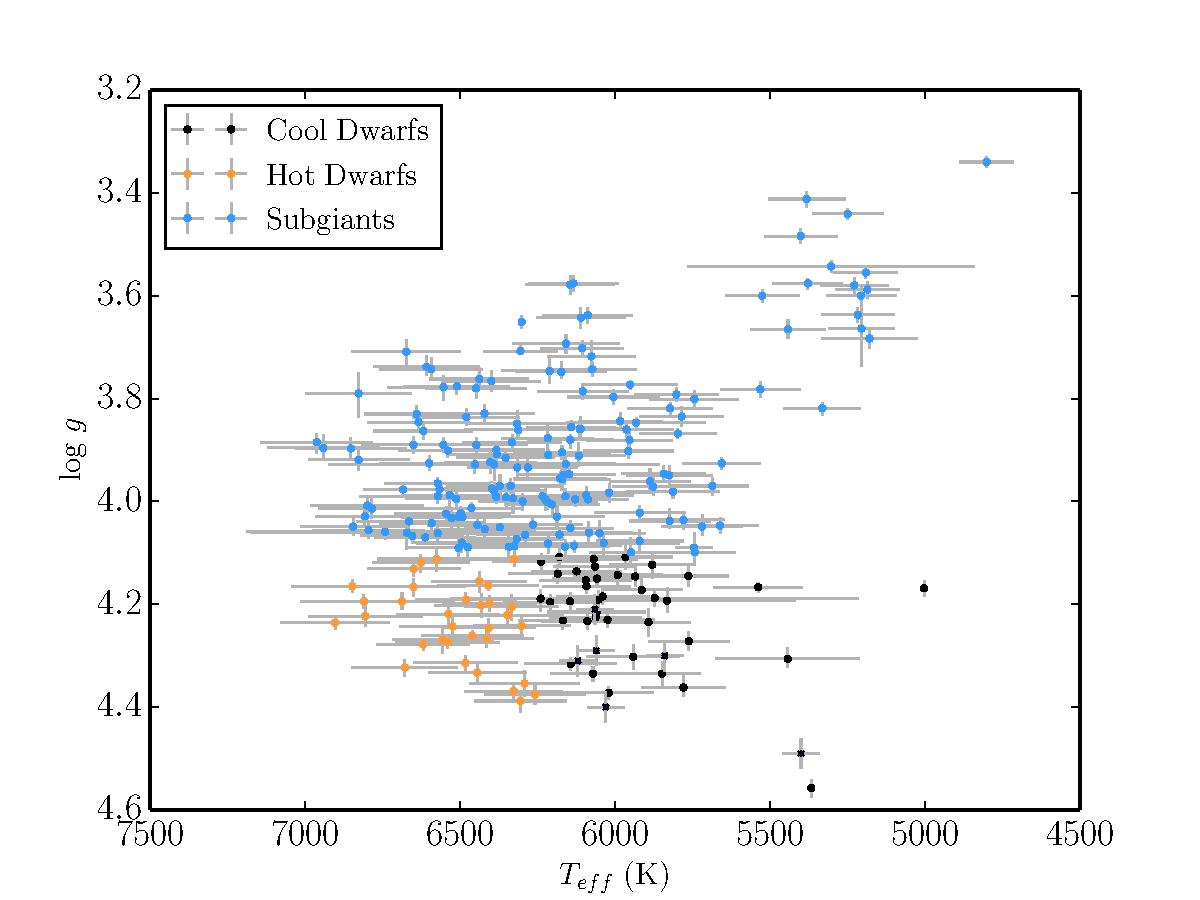
\includegraphics[width=6in, clip=true, trim=0 0 0.5in 0]{/Users/angusr/Python/Gyro/plots/logg_vs_t_paper.png}
\caption{\logg vs \teff for the 153 asteroseismic stars. Stars with \teff $>$ 6250 K are red and those with \logg $<$ 4.0 are blue. The triangular data points are those with precise ages. {\color{red}To do: add ASTEC isochrones}}
\label{fig:p_vs_a}
\end{center}
\end{figure}

\citet{Garcia2014} use a combination of wavelet transforms and ACFs to measure the surface rotation periods of Kepler asteroseismic stars.
They use a Morlet mother wavelet which is the convolution of a sinusoid and a Gaussian.
They require that at least four full rotation periods are present in the data
They use two sets of data: PDC-MAP and KADACS and two periodicity measurement methods: ACF and wavelet transform.
They require all four of these possible data and analysis method combinations to be consistent to within 20\%.
They then visually check the data.
compute a wavelet transform for each light curve and project it onto the period axis, reinforcing the true period and suppresing harmonic and sub-harmonic signals.
The details of this method are outlined in \citet{Mathur2014}.

\subsection{Observational data}

\citet{Chaplin2013} calculated the ages of 505 Kepler targets using the above scaling relations.
A grid-based approach was used to measure stellar properties: values of $\Delta\nu$ were calculated for each R and M on the grid and compared with the observed $\Delta\nu$.
Ages quoted in \citet{Chaplin2013} are the combined result of six different grid-based model pipelines.
The uncertainties on the ages reflect discrepancies between results obtained using different sets.
Two sets of effective temperatures were used: one was derived using an Infra-Red Flux Method (IRFM) calibration (\citealt{Casagrande2010}, \citealt{SilvaAguirre2012}) and the other from a recalibration of the SDSS griz filter KIC photometry by \citet{Pinsonneault2012} using Yale Rotating Stellar Evolution Code (YREC) models \citep{Demarque2004}.
We use the second set of temperatures since they are slightly more precise, however our analysis is relatively insensitive to this choice.
% test: is our analysis sensitive to this choice?

The asteroseismic ages in \citet{Chaplin2013} have typical uncertainties of $\sim$ 35\%; however, it will be possible to derive more precise ages for some of these stars.
By measuring the frequency of each oscillation mode individually, not just the mean large serparation, one can build up a density profile of the star and provide a tighter constraint on its age.
Ages derived from individual oscillation mode measurements can have uncertainties as small as 10\% (\citet{Brown1994}, \citet{SilvaAguirre2013}), however measuring frequencies for individual oscillation modes is a manual process and can only be applied in the highest signal-to-noise cases.
\citet{Chaplin2013} predict that around 150 of the 505 stars will be suitable for this individual oscillation mode treatment.
We obtained precise ages for 42 stars from \citet{Metcalfe2014}, modelled with the Asteroseismic Modeling Portal (AMP), with effective temperatures and metallicities from \citet{Bruntt2012}.
% Of the 42 stars in \citep{Metcalfe2014}, we only integrate the `simple stars' (cool dwarfs) into our sample---we ignore the `F stars' and `mixed mode' (subgiant) stars as these are not expected to follow the simple gyrochronology relation.
% {\color{red} Shouldn't I include these to be consistent?}

% Notes - apparently asteroseismic ages are easier to derive for older stars!
% We are calibrating the relation between period, age and colour---this is different to the relation between period, age and mass because
% colour-mass relation is different for different compositions and this adds a level of systematic uncertainty.
The asteroseismic sample covers a large range of ages (see figure \ref{fig:p_vs_a}), however it does not provide good mass coverage across the entire range.
There are very few stars with temperatures below 6000 K (B-V $\sim$ 0.55) and of the low mass stars, most of them are old (note---the paucity of massive, old stars is an effect of MS turn-off).
We therefore added 261 stars to our sample from young clusters Coma Berenices (0.5 Gyr), Praesepe (0.588 Gyr), the Hyades (0.625 Gyr) and NGC6811 (1.1 Gyr) (see table \ref{tab:clusters}).
We only added clusters with ages greater than 0.5 Gyrs as these younger clusters often have large populations of rapid rotators that have not yet converged onto the gyrochronology plane.

\begin{deluxetable}{lcccc}
\label{tab:clusters}
\tablewidth{0pc}
\tablecaption{Clusters and References: (1) \citet{Soderblom2009}, (2) \citet{Hartman2010}, (3) \citet{Jones1996}, (4) \citet{Meibom2011_M34}, (5) \citet{Dobbie2009}, (6) \citet{CollierCameron2009}, (7) \citet{Khalaj2013}, (8) \citet{Kovacs2014}, (9) \citet{Perryman1998}, (10) \citet{Radick1987}, (11) \citet{Janes2011}, (12) \citet{Meibom2011}. NGC 6811 g-r colours were converted to dereddened B-V with $E_{(B-V)}$ = 0.1. The age of M 34 reported in \citet{Jones1996} is 200-250 Myr.}
\tablehead{
\colhead{Cluster}&
\colhead{Age (Gyr)}&
\colhead{Number of stars}&
\colhead{Age ref}&
\colhead{Rotation period ref}}
\startdata
% Pleides & 0.1 $\pm$ 0.05 & 1 & 2 \\
% M 34 & 0.225 $\pm$ 0.025 & 3 & 4 \\
Coma Ber & 0.5 $\pm$ 0.1 & 28 & 5 & 6 \\
Praesepe & 0.588 $\pm$ 0.137 & 161 & 7 & 8 \\
Hyades & 0.625 $\pm$ 0.05 & 22 & 9 & 10\\
NGC 6811 & 1.1 $\pm$ 0.2 & 50 & 11 & 12 \\
\enddata
\end{deluxetable}

\begin{deluxetable}{lccc}
\label{tab:field_stars}
\tablewidth{0pc}
\tablecaption{Rotation periods and B-V colours for field stars with precise ages.
References: (1) \citet{Metcalfe2012}, (2) \citet{Henry2000}, (3) \citet{Moffet1979}, (4) \citet{Li2012}, (5) \citet{Petit2008}, (6) \citet{Mermilliod1986}, (7) \citet{Bouvier2010}, (8) \citet{Donahue1996}, (9) \citet{Cox2000}, (10) \citet{Bazot2012}, (11) \citet{Yildiz2007}, (12) \citet{Hallam1991}, (13) \citet{Dumusque2012}.}
\tablehead{
\colhead{ID}&
\colhead{age}&
\colhead{\prot}&
\colhead{B-V}}
\startdata
16 Cyg B & 6.4 $\pm$ 0.4$^1$ & 31.5 $\pm$ 6.5$^2$ & 0.66 $\pm$ 0.01$^3$ \\
18 Sco & 3.66 $\pm$ 0.2$^4$ & 22.7 $\pm$ 0.5$^5$ & 0.64 $\pm$ 0.01$^6$ \\
The Sun & 4.568 $\pm$ 0.001$^7$ & 26.09 $\pm$ 0.1$^8$ & 0.65 $\pm$ 0.001$^9$ \\
$\alpha$ Cen A & 6 $\pm$ 1$^{10,11}$ & 28.8 $\pm$ 2.5$^{12}$ & 0.69 $\pm$ 0.01$^6$ \\
$\alpha$ Cen B & 6 $\pm$ 1$^{10,11}$ & 38.7 $\pm$ 5.0$^{13}$ & 0.90 $\pm$ 0.01$^6$ \\
\enddata
\end{deluxetable}

\begin{figure}[ht]
\begin{center}
	\subfigure[$P_{rot}$ vs \teff]{
            \label{fig:p_vs_t}
	    \includegraphics[width=3in, clip=true, trim=0 0 0.5in 0]{/Users/angusr/Python/Gyro/plots/p_vs_t_paper.png}
        }
	\subfigure[$P_{rot}$ vs B-V colour]{
            \label{fig:p_vs_bv}
	    \includegraphics[width=3in, clip=true, trim=0 0 0.5in 0]{/Users/angusr/Python/Gyro/plots/p_vs_bv_paper.png}
        }
    \end{center}
    \caption{ Photometric rotation period vs effective temperature and B-V colour for 153 Kepler asteroseismic targets. \teff was converted to B-V using \citet{Sekigchi2000}.
     }
   \label{fig:subfigures}
\end{figure}

Rotation periods and B-V colours for the Hyades were obtained from \citet{Radick1987} and an age of 650 Myrs was adopted from \citet{Perryman1998}.
NGC 6811 is a cluster in the Kepler field with an age of 1.1 $\pm$ 0.2 Gyr \citep{Janes2011} with photometric rotation periods for cluster members measured by \citet{Meibom2011}.
These stars have g-r colours which were converted to dereddened B-V with $E_{(B-V)} = 0.1$.
Rotation periods for the 590 Myr \citep{Khalaj2013} cluster Praesepe were published in \citet{Kovacs2014}, with dereddened B and V colours from the APASS database ((http://www.aavso.org/apass).

A further 5 field stars with precise age measurements were added to the sample: 16 Cyg B, Alpha Cen A and B, 18 Sco and, of course, the Sun (see table \ref{tab:field_stars}).
An asteroseismic age for 16 Cyg B was obtained from \citet{Metcalfe2012}, $T_{eff}$ from \citet{Ramirez2009} and rotation period from \citet{Henry2000} with B and V colours from \citet{Moffett1979}.
An age of 6 $\pm$ 1 Gyr was adopted for Alpha Cen AB, based on the analysis by \citet{Bazot2012} and \citet{Yildiz2007} (note that ages derived for Alpha Cen AB are extremely model dependent).
B and V colours were obtained from \citet{Mermilliod1986} and rotation periods from \citet{Hallam1991} and \citet{Dumusque2012} for A and B, respectively.
An age of 4.568 $\pm$ 0.001 Gyr for the Sun was taken from \citet{Bouvier2010}, and a latitudinal mean rotation period, observed by \citet{Donahue1996}.
% We also include the Sun as an old anchor datum, adopting a period of 26.09 days which is the latitudinal mean observed by Donahue et al. (1996) (the solar rotation ranges from ø25 days near the equator to ø32 days near the poles).
The age of 3.66 $\pm$ 0.2 for 18 Sco was taken from \citet{Li2012}, with rotation period from \citet{Petit2008} and B and V colours from \citet{Mermilliod1986}.

Despite having effective temperatures for the asteroseismic targets, we converted $T_{eff}$ to B-V colours, using the relation in \citet{Sekiguchi2000}---see figure \ref{fig:subfigures}.
This conversion is imprecise since the metallicites of the asteroseismic targets are the field average and not calculated per star.
Eventually we intend to provide an effective temperature calibration in addition to this colour calibration.
% however we concluded that converting $T_{eff}$ to colour would be more efficient than converting cluster star colours to $T_{eff}$, since we have more information about the asteroseismic sample.

The entire set of 418 stars is shown in figure \ref{fig:3d}. Asteroseismic targets are shown in black, with supplementary cluster and field stars in red.

\begin{figure}[ht]
\begin{center}
\includegraphics[width=6in, clip=true, trim=0 0 0.5in 0]{/Users/angusr/Python/Gyro/plots/3d_angled.png}
\caption{Colour, age and rotation periods of all 418 stars. Asteroseismic stars are black and additional cluster and field stars are red. {\color{red}add precise stars.}}
\label{fig:3d}
\end{center}
\end{figure}

\begin{figure}[ht]
\begin{center}
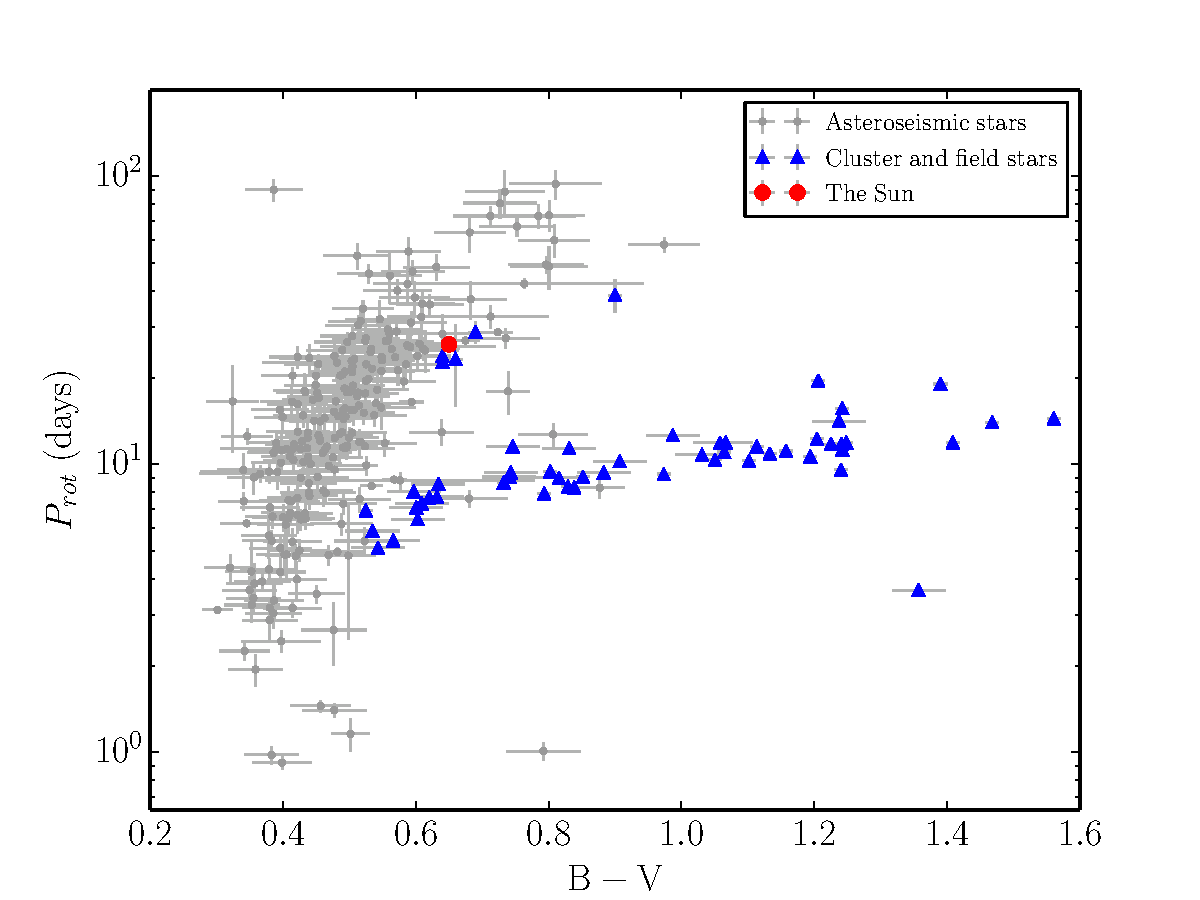
\includegraphics[width=6in, clip=true, trim=0 0 0.5in 0]{/Users/angusr/Python/Gyro/plots/p_vs_bv_paper2.png}
\caption{Photometric rotation period vs B-V colour for 153 Kepler targets (black) plus cluster and field stars (red). The blue stars have precise ages.}
\label{fig:3d}
\end{center}
\end{figure}

\begin{figure}[ht]
\begin{center}
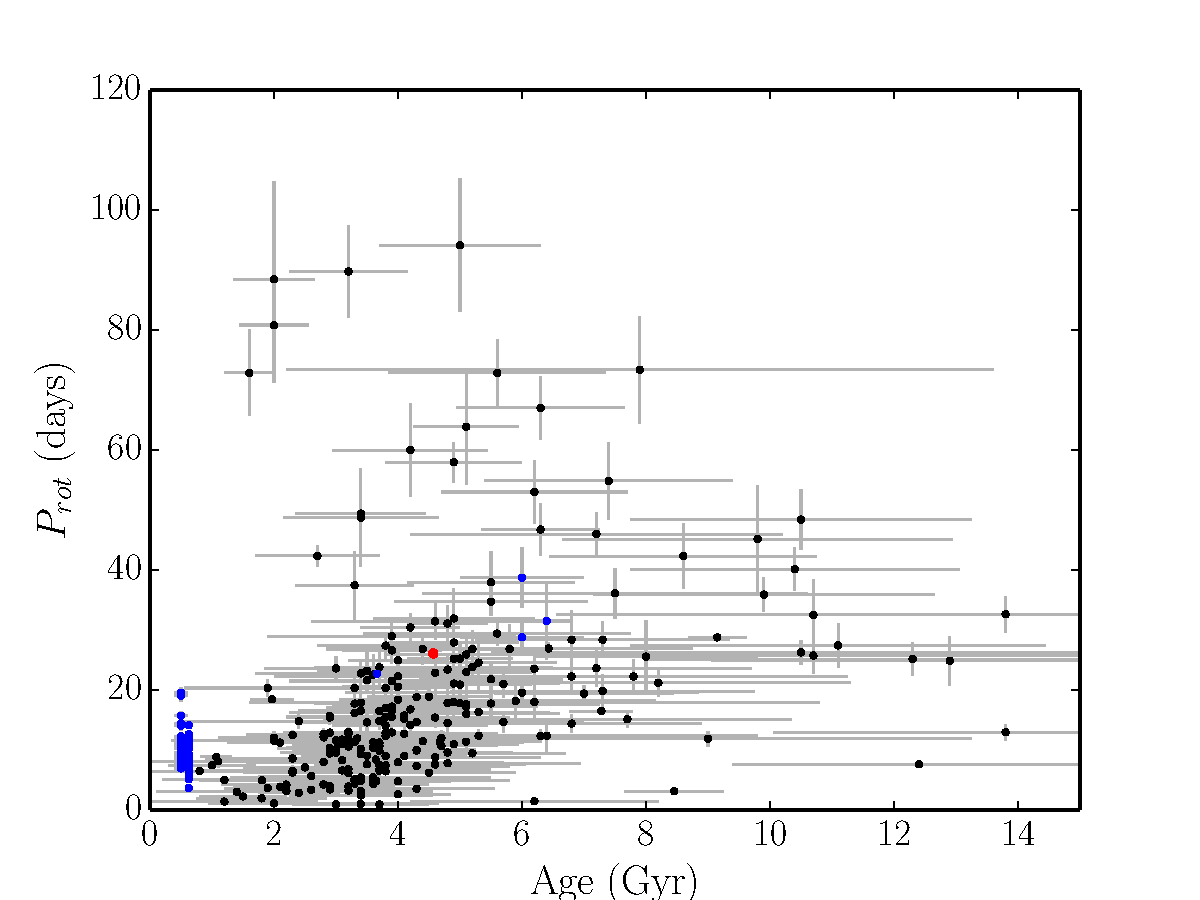
\includegraphics[width=6in, clip=true, trim=0 0 0.5in 0]{/Users/angusr/Python/Gyro/plots/p_vs_a_paper2.png}
\caption{Photometric rotation period vs age for 153 Kepler targets (black) plus cluster and field stars (red). The blue stars have precise ages. {\color{red} add 7 other precise stars.}}
\label{fig:p_vs_a}
\end{center}
\end{figure}

\bibliographystyle{plainnat}
\bibliography{Gyro_paper}

\end{document}
